\documentclass[fr]{../../../../../../eplexam}
\usepackage{../../../../../../eplunits}
\usepackage{circuitikz}
\usepackage{pgfplots}
\usepackage{enumitem}
\pgfplotsset{compat=newest}
\tikzset{meter/.style={draw,thick,circle,fill=white,minimum size =0.75cm,inner sep=0pt}}

\hypertitle{circmes-ELEC1370}{4}{ELEC}{1370}{2013}{Juin}
{Nicolas Verbeek\and Adrien Couplet\and Martin Van Essche\and Guillaume Gilson\and Guillaume Colinet}
{Claude Oestges, Bruno Dehez and Christophe Craeye}

\section{Question Oestges : phaseurs}
Soit le circuit suivant avec $V_o=5.5\angle\ang{104.1}$ V,
\begin{center}
    \begin{circuitikz} 
    	\draw
  		(0,-2.5) to[american voltage source,l=$6\angle\ang{0}$ V] (0,2.5) 
  		(2.5,2.5) to[european resistor,l=$Z$] (0,2.5)
  		(2.5,2.5) -- (5,2.5)
  		(2.5,0) to[L,i=$I_L$,l=j$\SI{2}{\ohm}$,-*] (2.5,2.5)
  		(2.5,0) to[R,v=$V_o$,l=$\SI{2}{\ohm}$] (2.5,-2.5)
 		(5,2.5) to[american current source,l=$2\angle\ang{0}$ A] (5,-2.5)
		(0,-2.5) -- (5,-2.5);
 	\end{circuitikz}
\end{center}
  
On demande de calculer
\begin{enumerate}
    \item Le courant $I_L$ dans l'inductance
    \item L'impédance $Z$ et les caractéristiques des composants ($R$,$L$,$C$) avec une fréquence de $f=\SI{10}{\kilo\hertz}$.
    \item La puissance active délivrée par la source de tension
    \item Le dipôle équivalent de Thévenin aux bornes de la résistance de $\SI{2}{\ohm}$.
    \item Le courant dans une résistance de $\SI{3}{\ohm}$ mise en série avec ce dipôle équivalent.
\end{enumerate}

\begin{solution}
\begin{enumerate}
    \item $I_L = 2.75\angle -75.9^\circ$ A
    \item $Z = 0.698-4.404j \Rightarrow R=\SI{0.7}{\ohm}$ et $C = \SI{3.614}{\micro\farad}$
    \item $P = \SI{4}{\watt}$
    \item $V_\text{th} = 9.94 \angle 62.41^\circ$ et $Z_\text{th} = Z+2j$
    \item $I = 2.25 \angle 95.45^\circ$ A
\end{enumerate}
\end{solution}

\section{Question Dehez : triphasé}
Soit le circuit suivant
\begin{center}
    \begin{circuitikz}[scale=0.9]
        \coordinate (s1) at (0,0);
        \coordinate (s2) at ($ (s1) + ({3*cos(60)},{-3*sin(60)}) $);
        \coordinate (s3) at ($ (s1) + ({-3*cos(60)},{-3*sin(60)}) $);
        
        \draw (s1) to[V,l=$34\angle\ang{0}\,\si{\volt}$,i=$I_1$,*-*] (s2) to [V,l=$34\angle\ang{-120}\,\si{\volt}$,-*] (s3) to [V,l=$34\angle\ang{-240}\,\si{\volt}$] (s1);
        \draw (s1) to [R,l=\SI{2}{\ohm}] ++(5,0) coordinate (l11); 
        \draw (s3) to[short] ++(0,-2) coordinate (p1);
        
        \coordinate (l12) at ($ (l11) + ({3*cos(60)},{-3*sin(60)}) $);
        \coordinate (l13) at ($ (l11) + ({-3*cos(60)},{-3*sin(60)}) $);
        \coordinate (c1) at ($ (l11) + (0,{-sqrt(3)}) $);
        
        \draw (l11) to[L,l_=\SI{j}{\ohm},-*] (c1);
        \draw (c1) to[L,l=\SI{j}{\ohm}] (l12);
        \draw (c1) to[L,l_=\SI{j}{\ohm}] (l13);
        
        \draw (l13) to[R,l=\SI{2}{\ohm}] (s2);
        \draw (l12) to[short] ++(0,-2) to[R,l=\SI{2}{\ohm}] (p1);
        
        \coordinate (l21) at ($ (l11) + (3.5,0) $);
        \coordinate (l22) at ($ (l21) + ({3*cos(60)},{-3*sin(60)}) $);
        \coordinate (l23) at ($ (l21) + ({-3*cos(60)},{-3*sin(60)}) $);
        \coordinate (c2) at ($ (l21) + (0,{-sqrt(3)}) $);
        
        \draw (c2) to[L,l_=\SI{8j}{\ohm},*-] (l21);
        \draw (c2) to[L,l=\SI{8j}{\ohm}] (l22);
        \draw (c2) to[L,l_=\SI{8j}{\ohm}] (l23);
        
        \coordinate (d1) at ($ (l21) + (3.5,0) $);
        \coordinate (d2) at ($ (d1) + ({3*cos(60)},{-3*sin(60)}) $);
        \coordinate (d3) at ($ (d1) + ({-3*cos(60)},{-3*sin(60)}) $);
        \draw (d3) to[short] ++(0,-1) coordinate (p2);
        \draw (d2) to[short] ++(0,-2) coordinate (p3);
        \draw (l21) to[short] (d1);
        \draw (l23) to[short] ++(0,-1) to[short] (p2);
        \draw (l22) to[short] ++(0,-2) to[short] (p3);
        \draw (d1) to[C,l=\SI{-3j}{\ohm},i=$I_2$,*-*] (d2) to[C,l=\SI{-3j}{\ohm},-*] (d3) to[C,l=\SI{-3j}{\ohm}] (d1);
        
        \draw (l11) node[below left]{$\bullet$};
        \draw (l21) node[below right]{$\bullet$};
        \draw (l12) node[above]{$\bullet$};
        \draw (l22) node[below left]{$\bullet$};
        \draw (l13) node[below right]{$\bullet$};
        \draw (l23) node[above]{$\bullet$};
        \draw [<->,>=stealth] ($ (l11) + (-0.2,0.2) $)  to [bend left] node[pos=0.5,above] {\SI{6j}{\ohm}} ($ (l21) + (0.2,0.2) $);

    \end{circuitikz}
\end{center}
\begin{enumerate}
    \item Calculer le facteur de dispersion du couplage magnétique;
    \item Calculer l'amplitude et la phase de $I_1$ et $I_2$.
\end{enumerate}

\begin{solution}
\begin{enumerate}
    \item $$1- \sigma  = 1- \frac{M^2}{L_1 L_2} = -3.5$$
    On a ici un facteur de dispersion négatif (impossible physiquement mais erreur de Mr. Dehez. \textit{Errare humanum est}.)
    \item On commence par la transformation des sources et des capacités en modèle étoile.\\ Après cette transformation, on a :
    \begin{itemize}
        \item $V_s = \frac{34}{\sqrt3} \angle\ang{-30}$ [V]
        \item $j\omega C = -j$ [$\Omega$]
    \end{itemize}
    On passe en monophasé, on trouve un courant $I_1'$ dans la partie de gauche égal à $4.267\angle 34.2^\circ$ [A]. On trouve un courant $I_2 = 3.657 \angle34.23^\circ$ [A]. \\
    Connaissant $I_{1}'$ (courant de ligne) on peut trouver le courant $I_{1}$ (courant de phase) via la relation liant les 2 grandeurs.
    On trouve $I_1 = 2.464 \angle 64.23^\circ$ [A].
\end{enumerate}
\end{solution}

\section{Question Craeye : transitoire}
Soit le circuit commuté ci-dessous. Donnez l'expression temporelle de la tension $V_c$ pour $t>0$ (l'interrupteur passe de la borne $A$ à la borne $B$ en $t=0$). Les valeurs des éléments du circuits sont: $R_o = R_1 = R = \SI{1}{\kilo\ohm}$, $C=\SI{1}{\nano\farad}$ et $L_o = L = \SI{1}{\milli\henry}$.
\begin{center}
    \begin{circuitikz}
        \draw (0,0) to[american voltage source,l=\SI{1}{\volt}] ++(0,4) to[R,l=$R_1$] ++(0,4) to[short,-o] ++(1,0) coordinate (B);
        \draw (2,8) to[short] ++(2,0) to[R,l=$R$] ++(2,0) to[L,l=$L$] ++(0,-8) to[short] ++(-6,0);
        \draw (2,0) to[american voltage source,l=\SI{2}{\volt}] ++(0,2) to[L,l=$L_o$] ++(0,2) to[R,l=$R_o$] ++(0,2) to[short,-o] ++(0,1) coordinate (A);
        \draw (1.4,7.4) to[short,o-] (2,8);
        \draw (4,0) to[short] ++(0,3) to[C,l=$C$,v>=$V_c$] ++(0,2) to[short] ++(0,3);
        
        \draw [->,>=stealth] ($ (A) + (-0.2,0) $)  to [bend left] node[pos=0.5,below left] {$t=0$} ($ (B) + (0,-0.2) $);
        \draw (A) node[right]{$A$};
        \draw (B) node[above]{$B$};
    \end{circuitikz}
\end{center}

\begin{solution}
\[V_c(t) = \frac{1}{2} + \frac{1}{2}e^{-10^6t}(\cos(10^6t)-\sin(10^6t))\]
ou la solution équivalente avec seulement un cosinus
\[ V_c(t) = \frac{1}{2} + 0.707 e^{-10^6t}\cos(10^6t+0.785) \]

\begin{center}
    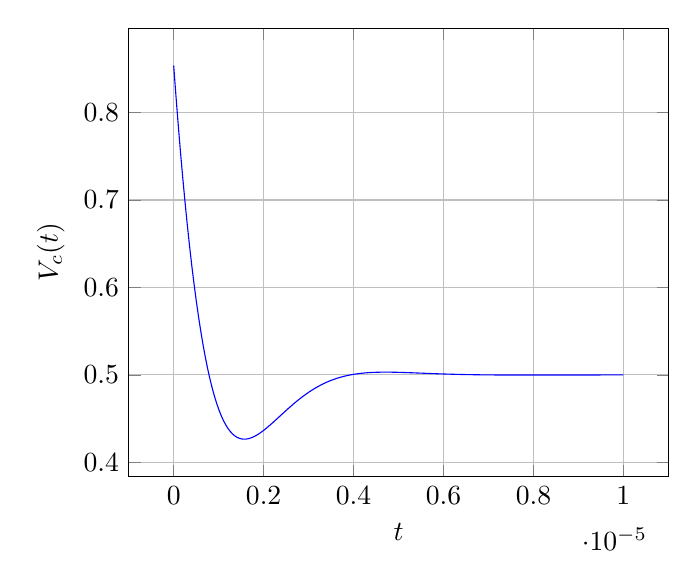
\begin{tikzpicture}
        \begin{axis}[enlargelimits=true,grid=major,ylabel=$V_c(t)$,xlabel=$t$]
            \addplot [blue,domain=0:0.00001,samples=200]{0.5 + 0.5*e^(-(10^6)*x)*cos(deg(10^6*x + 0.785))};
        \end{axis}
    \end{tikzpicture}
\end{center}
\end{solution}

\end{document}
